 \begin{itemize}
		\item {\textbf{Kratak opis:} Nakon uspeshne obrade porud2bine administrator dostavlja vozachu informacije potrebne za proces 			dostavljanja(kolichinu robe, destinaciju za dostavljanje, potvrdu narud2bine). Nakon vozachovog dolaska u skladishte i uspeshnog utovara kolichine robe koja je potrebna. Vozach obaveshtava administratora o pochetku procesa dostavljanja i upuc1uje se ka destinaciji. U sluchaju pravljenja pauze , vozach obaveshtava administratora o tipu pauze, koja mozhe biti Nakon vozachevog dolaska na destinaciju dostavljanja, vozach shalje potvrdu administratoru o pristizanju na zheljenu destinaciju. I proces istovara i naplate mozhe da pochne.}
		\item{\textbf{Ucesnici:} Vozach, Administrator}
		\item{\textbf{Preduslovi:}  Najamnici u kamion utovaraju propisanu  kolichinu robe }
		\item{\textbf{Postuslovi:}  Roba je spremna za isotvar}
		\item{\textbf{Osnovni tok:}  
			\begin{enumerate}
				\item{Vozach administratoru shalje zahtev za pochetak transporta}
				\item{Administrator validira vozachev zahtev}
				\item{Administrator shalje vozachu dozvolu pochetka transporta}
				\item{Vozach zapochinje transport }
				\item{Vozach uspeshno zavrshava transport do odred1ene destinacije}
				\item {Vozach administratoru shalje potvrdu o zavrshenom transportu}
		\end{enumerate}}
	\item{\textbf{Alternativni tok:} 
		 \begin{itemize}
			\item[A{1}]{\textbf{Vozach pravi pauzu}
				 \begin{itemize}
					\item[A{1.1}] {Nuzhna pauza nakon koje vozach nastavlja putovanje}
					\item[A{1.2}] {Nezgoda , izvrshava se pomoc1ni tok  \textbf{P{1}}}
				\end{itemize}
								} 
			\item[A{2}] {\textbf{Vozachu nije dozvoljen polazak} 
				\begin{itemize}
					\item[A{2.1}]{Ne postoje moguc1nosti da se zahtevi ispune usled promena u sistemu , izvrshava se sluchaj upotrebe 2.3}
				\end{itemize}		
		
	}
		\end{itemize}
					}

	\item{\textbf{Podtokovi:}
		\begin{itemize}
			\item[P{1}]{\textbf{Dogodila se nezgoda na putu }
				\begin{enumerate}
					\item{Vozach obaveshtava administratora o nezgodi}
					\item{Administrator obaveshtava logistichare i servisere ako za to ima potrebe}
					\item{Izvrshava se Sluchaj Upotrebe 2.4}
				\end{enumerate}
							}
		\end{itemize}
			}
	\item{\textbf{Specijalni zahtevi:} \begin{itemize}
			\item[S{1}]{Vozach poseduje ured1aj kojim mozhe da komunicira sa administratorom}
			\item[S{2}]{Podrazumeva se da vozach uspeshno shalje zahteve administratoru i da ih on uspeshno prima}
			\item[S{3}]{Vozachev dolazak na destinaciju nije ukljuchen u sistem, podrazumeva se da se nalazi na destinaciji}
			\item[S{4}]{Vozach administratoru shalje obaveshtenje kada istovar zapochne}
		\end{itemize}}
	\item{\textbf{Dodatne informacije:}
			\begin{itemize}
				\item[D{1}]{Vozach se identifikuje jedinstvenim brojem vozacha koji je vezan za broj kamiona}
				\item[D{2}]{Unutar zahteva za pochetak transporta vozach prilazhe trenutno stanje natovarene robe kao i procenjeno vreme dolaska}
			\end{itemize}
		}
\end{itemize}
\begin{figure}[h!]
	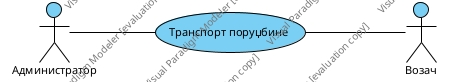
\includegraphics[scale=0.5]{Slike/UML/SUdostavljanjePorudzbineUseCase}
	\centering
	\caption{Dijagram sluchaja upotrebe:Transport porud2bine}
	\label{ucDostavljanje}
\end{figure}
\begin{figure}[h!]
	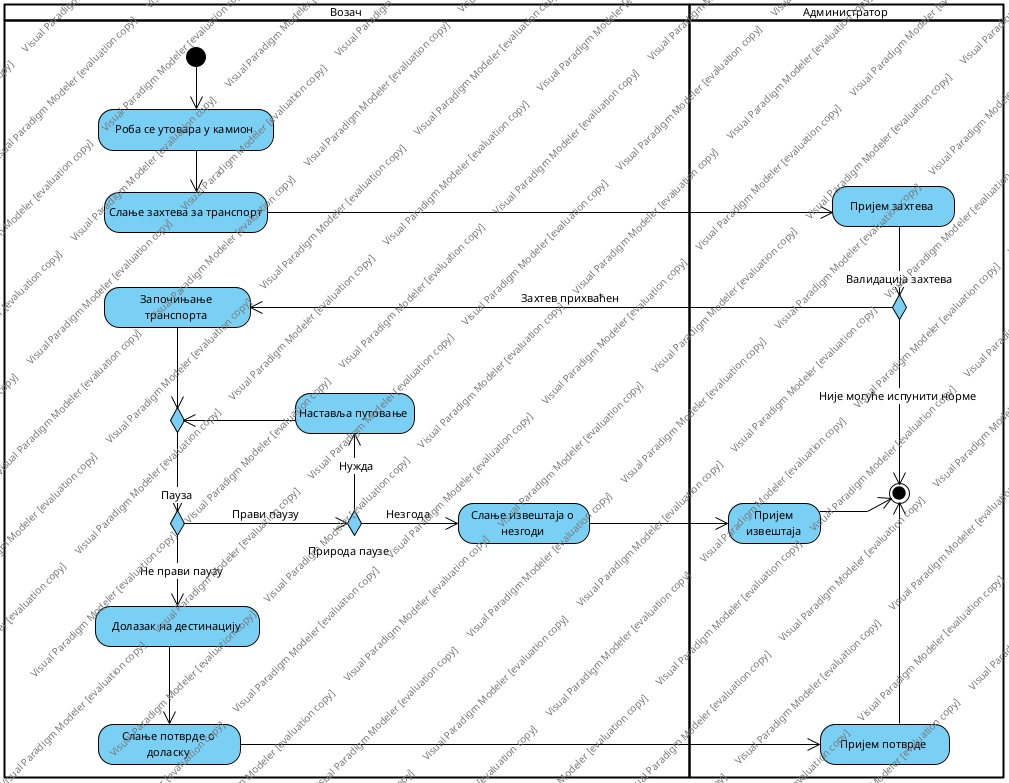
\includegraphics[scale=0.4]{Slike/DFD/SUdostavljanjePorudzbineActivity}
	\centering
	\caption{Dijagram aktivnosti :Transport porud2bine}
	\label{ucDostavljanjeAktivnost}
\end{figure}
\begin{figure}[h!]
	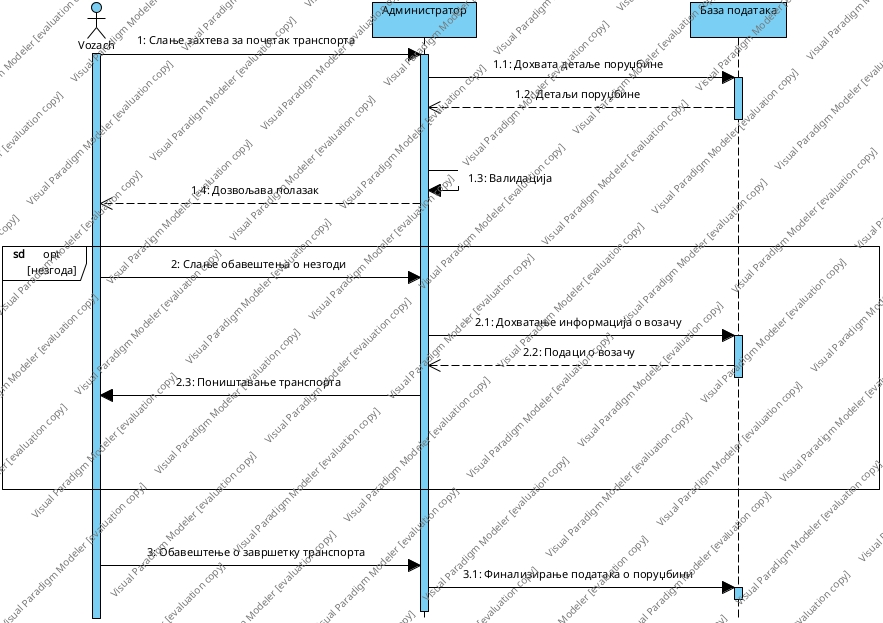
\includegraphics[scale=0.4]{Slike/DFD/SUdostavljanjePorudzbineDijagram Sekvenci.jpg}
	\centering
	\caption{Dijagram sekvencii :Transport porud2bine}
	\label{ucDostavljanjeSekvence}
\end{figure}
\begin{figure}[h!]
	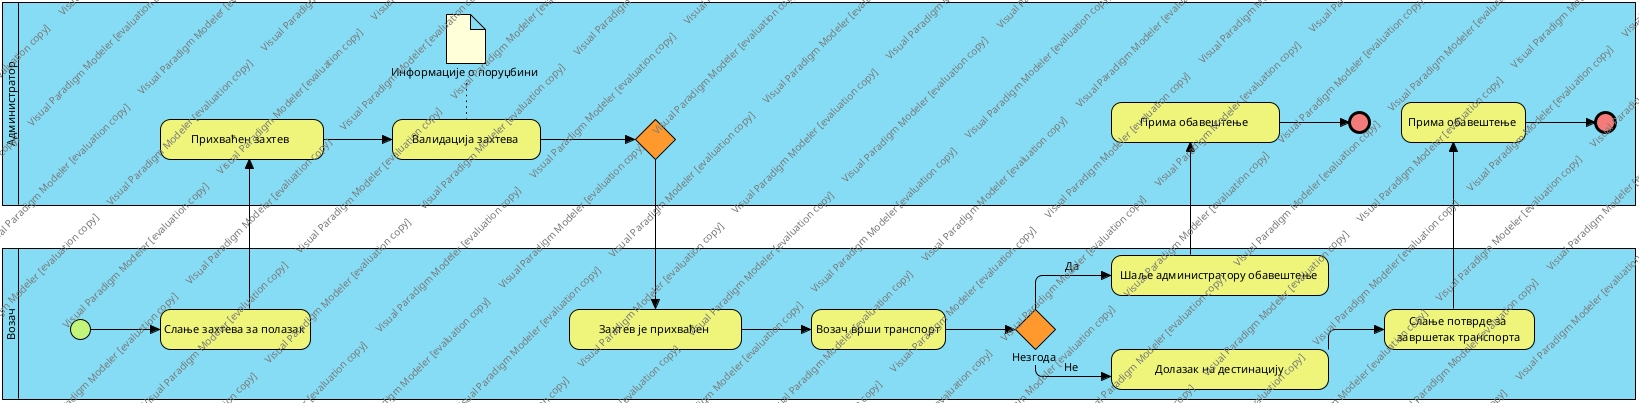
\includegraphics[scale=0.28]{Slike/BPMN/SUdostavljanjePorudzbineBPMN.jpg}
	\centering
	\caption{Dijagram BPMN :Transport porud2bine}
	\label{ucDostavljanjeBPMN}
\end{figure}







